\documentclass[a4paper]{article}

\usepackage[english]{babel}
\usepackage[utf8x]{inputenc}
\usepackage{amsmath}
\usepackage{graphicx}
\usepackage[colorinlistoftodos]{todonotes}

%_____________________________________________________________________________________
% THIS SOME THING THAT WILL GET OUR FIGURES IN THE RIGHT PLACE TAKEN FROM THE INTERNET ON THE WEBPAGE; http://mintaka.sdsu.edu/GF/bibliog/latex/floats.html

%%% START %%%
% Alter some LaTeX defaults for better treatment of figures:
    % See p.105 of "TeX Unbound" for suggested values.
    % See pp. 199-200 of Lamport's "LaTeX" book for details.
    %   General parameters, for ALL pages:
    \renewcommand{\topfraction}{0.9}	% max fraction of floats at top
    \renewcommand{\bottomfraction}{0.8}	% max fraction of floats at bottom
    %   Parameters for TEXT pages (not float pages):
    \setcounter{topnumber}{2}
    \setcounter{bottomnumber}{2}
    \setcounter{totalnumber}{4}     % 2 may work better
    \setcounter{dbltopnumber}{2}    % for 2-column pages
    \renewcommand{\dbltopfraction}{0.9}	% fit big float above 2-col. text
    \renewcommand{\textfraction}{0.07}	% allow minimal text w. figs
    %   Parameters for FLOAT pages (not text pages):
    \renewcommand{\floatpagefraction}{0.7}	% require fuller float pages
	% N.B.: floatpagefraction MUST be less than topfraction !!
    \renewcommand{\dblfloatpagefraction}{0.7}	% require fuller float pages

	% remember to use [htp] or [htpb] for placement
    
%%% END %%%
%_____________________________________________________________________________________

% NEEDED FOR THE REFERENCE
 %_______SOURCE; 

% START
\usepackage{hyperref}
% END





\title{Design and Control of a Lego Unicycle}
\author{Group B: Johan Kellerth Fredlund | Koshin Aliabase\\ Santiago Castro Chans | Sadik Kenan Sulejmanovic}

\begin{document}
\maketitle

\begin{abstract}
Your abstract.
\end{abstract}

\tableofcontents

\section{Author's note}

\section{Introduction}

Your introduction goes here! Some examples of commonly used commands and features are listed below, to help you get started. If you have a question, please use the help menu (``?'') on the top bar to search for help or ask us a question.

\section{Construction}

	\subsection{Ev3}
    \subsection{Sensors}
    	\subsubsection{HighTechinic Gyro Sensor}
        The Gyro sensor gives the rate of change in x, y and z orientation in radians per second. More specified details about the sensor can be seen in the table \ref{table:Gyro_sensor}. The first row shows how long time it takes for our program to fetch a sample, second row shows how accurate the sensor is given by specification by the manufacturer and the last line shows the update time of the sensor also given by the manufacturer. 
\\In nature all gyroscopes has a drift and offset, both are unwanted. The drift means that the rate of change will increase with time even though the sensor is stationary as can been observed in the figure \ref{fig:Gyro_offsets_refresh_times}. Secondly the offset is the property that give a constant value although the sensor is stationary. How we dealt with these problems will be explained in later sections. Lastly can we see the gyro sensor in figure \ref{fig:NXT_Gyro_Sensor}.  
        
        
        % THE TABLE DESCRIBING THE PROP. of the gyro sensor
        \begin{table}[h]
		\center
		\begin{tabular}{|c |c|}
			\hline
			 Refresh time in program & 10 ms (average)   \\ 
			\hline
			Accuracy &  $\pm 1$ degree \cite{NXT_Gyro_Sensor} \\ 
			\hline
			Update of value & 300 times / second  \cite{NXT_Gyro_Sensor} \\
	        		\hline
		\end{tabular}
		\caption{Specifications for the gyro under the name NXT Gyro Sensor (NGY1044).}
		\label{table:Gyro_sensor}
	\end{table}


	\begin{figure}[h]
		\centering
		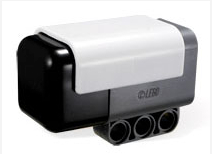
\includegraphics[width=0.3\textwidth]{NXT_Gyro_Sensor}
		\caption{Shows the gyro sensor which was used in the project.}
		\label{fig:NXT_Gyro_Sensor}
	\end{figure}
	
	\begin{figure}[h]
		\centering
		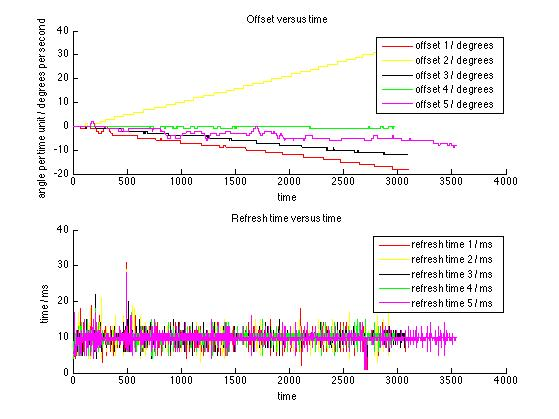
\includegraphics[width=1.3\textwidth]{plot_gyro_test_final_20150107}
		\caption{Shows the gyro sensor's offsets and refresh times when beeing stationary.}
		\label{fig:Gyro_offsets_refresh_times}
	\end{figure}
	
	\newpage
        
        
        \subsubsection{HighTechinic Accelerometer Sensor}
        
The accelerometer measure acceleration in x, y and z direction relative to the sensors specified directions given by the manufacturer. The specifications of the accelerometer can be seen in the table \ref{table:Acce_sensor} which shows the the time for it to give a sample to our program respectively number of times the sensor can update a value. On the other hand this sensor also comes with unwanted properties which is that the value is (very) noise however when it is not noise it gives reasonable good data. We can also see how this sensor looks like in the figure \ref{fig:NXT_Acce_Sensor} and the refresh time for a longer of time can be seen in the figure \ref{fig:plot_acce_refresh_time}
         % THE TABLE DESCRIBING THE PROP. of the Acce sensor
         \begin{table}[h]
		\center
		\begin{tabular}{|c |c|}
			\hline
			 Refresh time in program & 20 ms (average)   \\ 
			\hline
			Update of value &  100 times / second \cite{NXT_Acce} \\ 
			\hline
		\end{tabular}
		\caption{Specifications for the accelerometer under the name NXT Acceleration (NAC1040).}
		\label{table:Acce_sensor}
	\end{table}
	
	\begin{figure}[h]
		\centering
		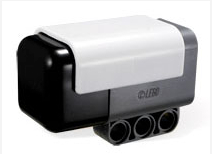
\includegraphics[width=0.3\textwidth]{NXT_Gyro_Sensor}
		\caption{Shows the accelerometer sensor which was used in the project.}
		\label{fig:NXT_Acce_Sensor}
	\end{figure}
	
	\begin{figure}[h]
		\centering
		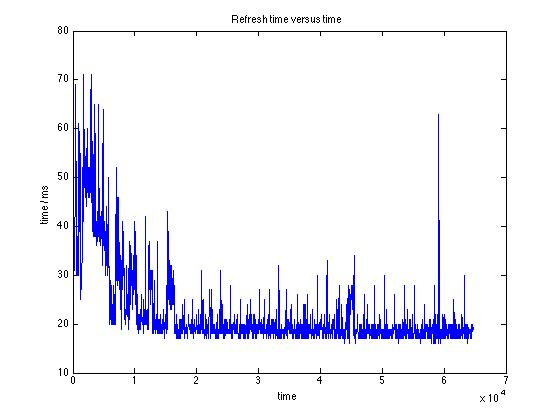
\includegraphics[width=1.3\textwidth]{plot_acce_refresh_time_20150107}
		\caption{Shows the accelerometer sensor refresh time.}
		\label{fig:plot_acce_refresh_time}
	\end{figure}
	
	
         
        
        
        \subsubsection{AbsoluteIMU-ACG}
        The AbsoluteIMU-ACG can gives gyro, accelerometer and compass data but in this project we are only interested in the gyro and the accelerometer therefor we will only discuss those measurements. As discussed previously gives the gyro part the rate of change in x,y and z. The accelerometer part measures the gravity in the x,y and z direction. The interesting part of this sensor is the refresh time versus the previous sensors and the update time can be seen in the figure \ref{fig:plot_IMU_sensor_sensitivity_0}. With this sensor one can also choose to have a smoothing filter for the accelerometer part of the IMU, downside is that this will increase the refresh time of the sensor. Therefor we did two measurements, one with sensitivity 0 and one with sensitivity 4 (figure \ref{fig:plot_IMU_sensor_sensitivity_4}). 
        
        \begin{figure}[h]
		\centering
		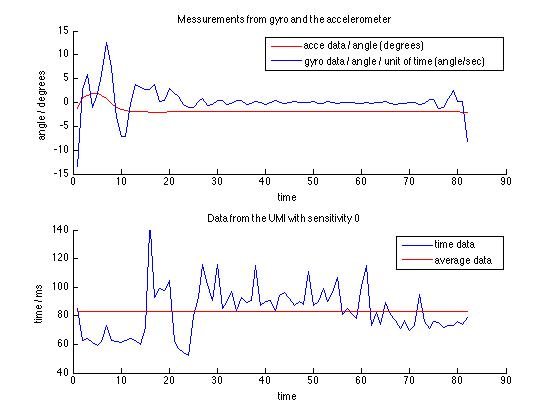
\includegraphics[width=1.3\textwidth]{plot_data_UMI_sen_0_20150103}
		\caption{Shows the important properties of the IMU sensor with sensitivity 0.}
		\label{fig:plot_IMU_sensor_sensitivity_0}
	\end{figure}
	
	      \begin{figure}[h]
		\centering
		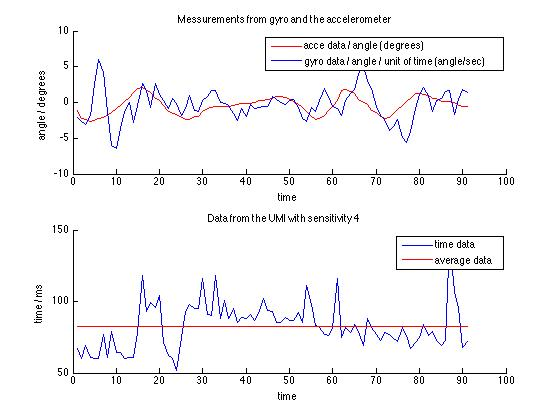
\includegraphics[width=1.3\textwidth]{plot_data_UMI_sen_4_20150107}
		\caption{Shows the important properties of the IMU sensor with sensitivity 4.}
		\label{fig:plot_IMU_sensor_sensitivity_4}
	\end{figure}
	
	
	\begin{table}[h]
		\center
		\begin{tabular}{|c |c|}
			\hline
			 Refresh time in program &  83 ms (average)   \\ 
			\hline
			Update of value &  100 times / second  \cite{IMU_sensor} \\ 
			\hline
		\end{tabular}
		\caption{Specifications for the IMU-ACG sensor.}
		\label{table:IMU_sensor}
	\end{table}
	
        
        
    \newpage 
    \subsection{Reaction wheel}
    
    
    
    
    \newpage
    \subsection{Motors}
    	\subsubsection{EV3 Large Servo Motor}
	This is one of the strongest motors there is for LEGO and the specifications for this motor can be seen in the table \ref{table:EV3_Large_servo_motor}. One experiment was done to get the connection between the torque and the power which is the parameter that control the PWM that goes to the motor. The power goes from -100 to 100. The result can be seen in the figure \ref{fig:plot_power_torque}.
	\cite{kinaSUR}
    
       \begin{figure}[h]
		\centering
		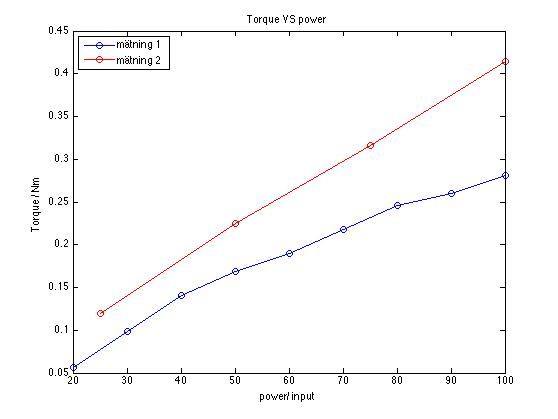
\includegraphics[width=1.3\textwidth]{plot_torque_versus_power_20151207}
		\caption{Shows the relation between the power and the torque of the motor.}
		\label{fig:plot_power_torque}
	\end{figure}
	
	\begin{table}[h]
		\center
		\begin{tabular}{|c |c|}
			\hline
			 RPM &  160 - 170  \cite{Ev3_Large_Servo_Motor}  \\ 
			\hline
			Running torque &  20 N/cm \cite{Ev3_Large_Servo_Motor}  \\ 
			\hline
			Stall torque  &  40 N/cm  \cite{Ev3_Large_Servo_Motor}  \\
			\hline
		\end{tabular}
		\caption{Specifications for the EV3 large motor server.}
		\label{table:EV3_Large_servo_motor}
	\end{table}
	
	
    
    
    \subsection{Prototypes}

\section{Modeling}
	\subsection{Lateral Balance}
		\subsubsection{Mathematical model}
        \subsubsection{Simulink model}
    \subsection{Medial Balance}
		\subsubsection{Mathematical model}
        \subsubsection{Simulink model}
        
\section{Implementation}
	\subsection{Programs}
    	\subsubsection{Lejos}
    	\subsubsection{NXC}
    \subsection{Sensors}
    
\section{Results}

\section{Discussion and Conclusion}




% NEDED FOR THE REFERENCE, PART 2
% SOURCE;    
% START
\bibliographystyle{plain}
\bibliography{ref_bib}	% d�r "ref_bib" �r "ref_bib.bib" filen i samma mapp d�r alla referenser defineras 
% END
\end{document}